\subsection{SEIR模型}
\paragraph{考虑病毒潜伏期,在$SIR$模型的基础上加入病毒携带者人群,即为$SEIR$模型:}
\begin{itemize}
	\item 人群
	      \subitem $S$:易感者
	      \subitem $I$:感染者
	      \subitem $R$:康复者
	      \subitem $E$:携带者
	\item 感染机制
	      \subitem
	      \begin{align}
		      \TP{S}{E}{S(I+E)} \\
		      \TP{E}{I}{E}      \\
		      \TP{I}{R}{I}
	      \end{align}
	      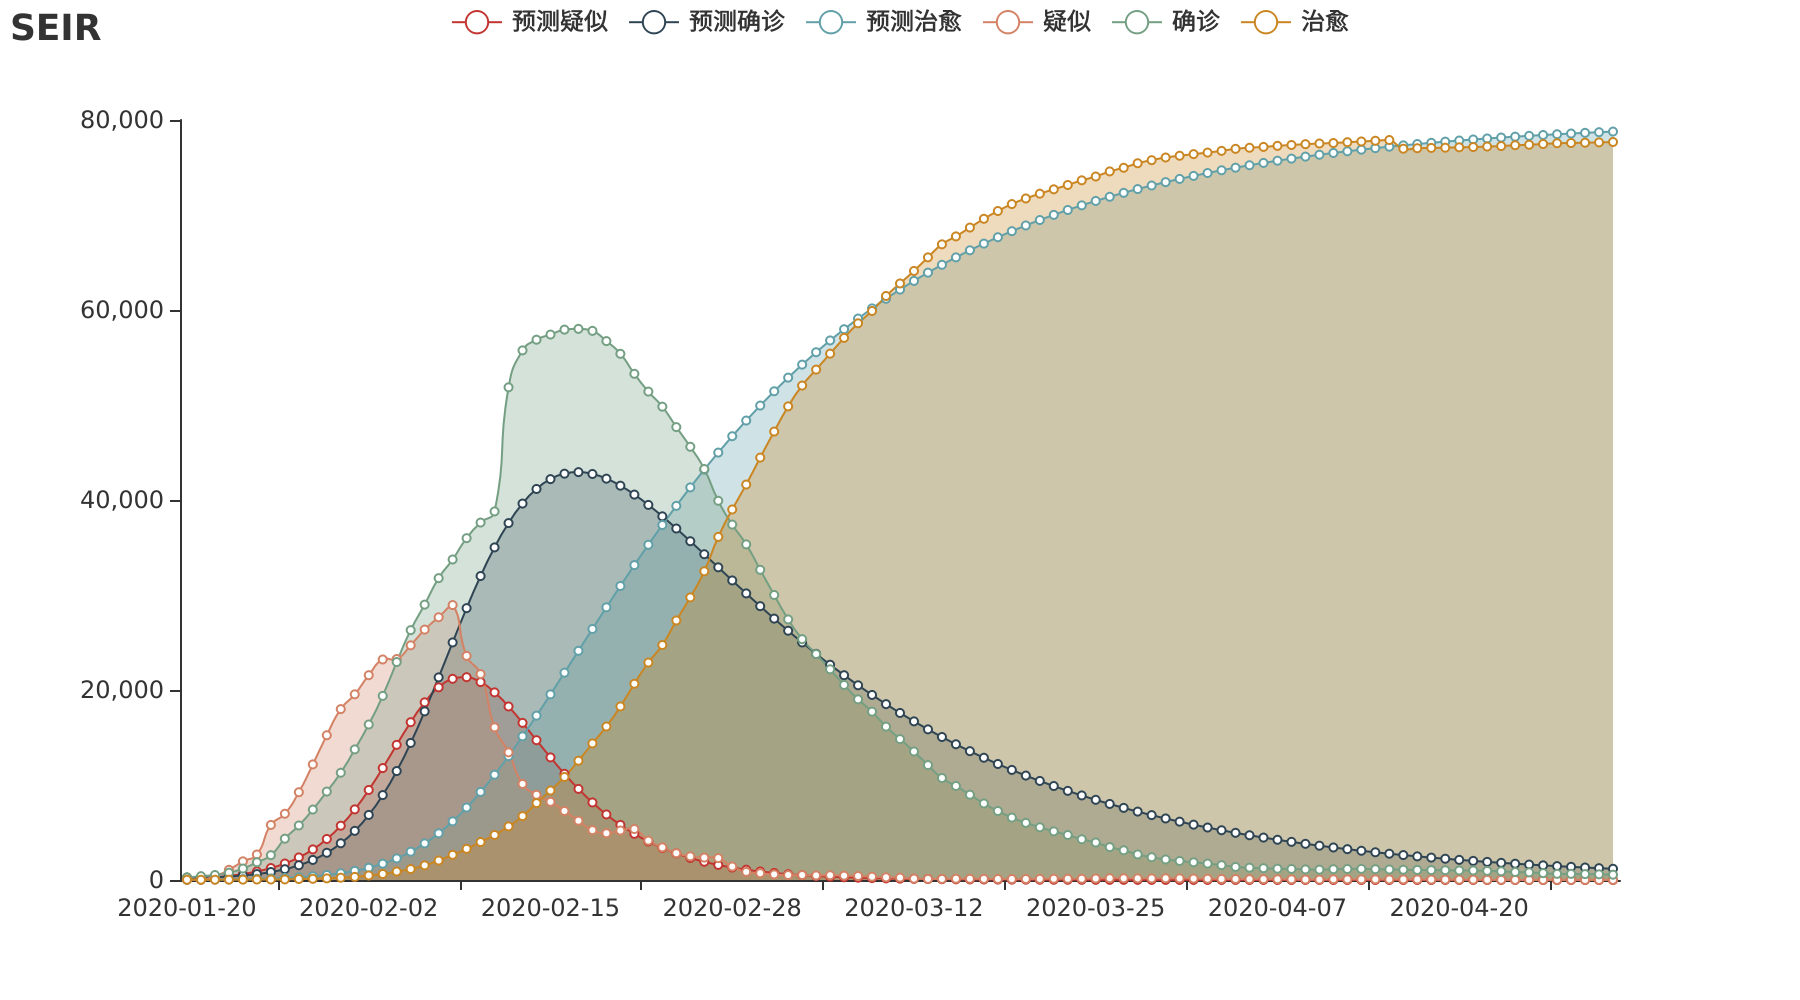
\includegraphics[width=.9\textwidth]{SEIR.png}
\end{itemize}
\subsection{SEIRD模型}
考虑死亡人群
\begin{itemize}
	\item 人群
	      \subitem $S$:易感者
	      \subitem $I$:感染者
	      \subitem $R$:康复者
	      \subitem $E$:携带者
	      \subitem $D$:病逝者
	\item 感染机制
	      \subitem
	      \begin{align}
		      \TP{S}{E}{S(I+E)} \\
		      \TP{E}{I}{E}      \\
		      \TP{E}{R}{E}      \\
		      \TP{I}{R}{I}      \\
		      \TP{I}{D}{I}
	      \end{align}
	      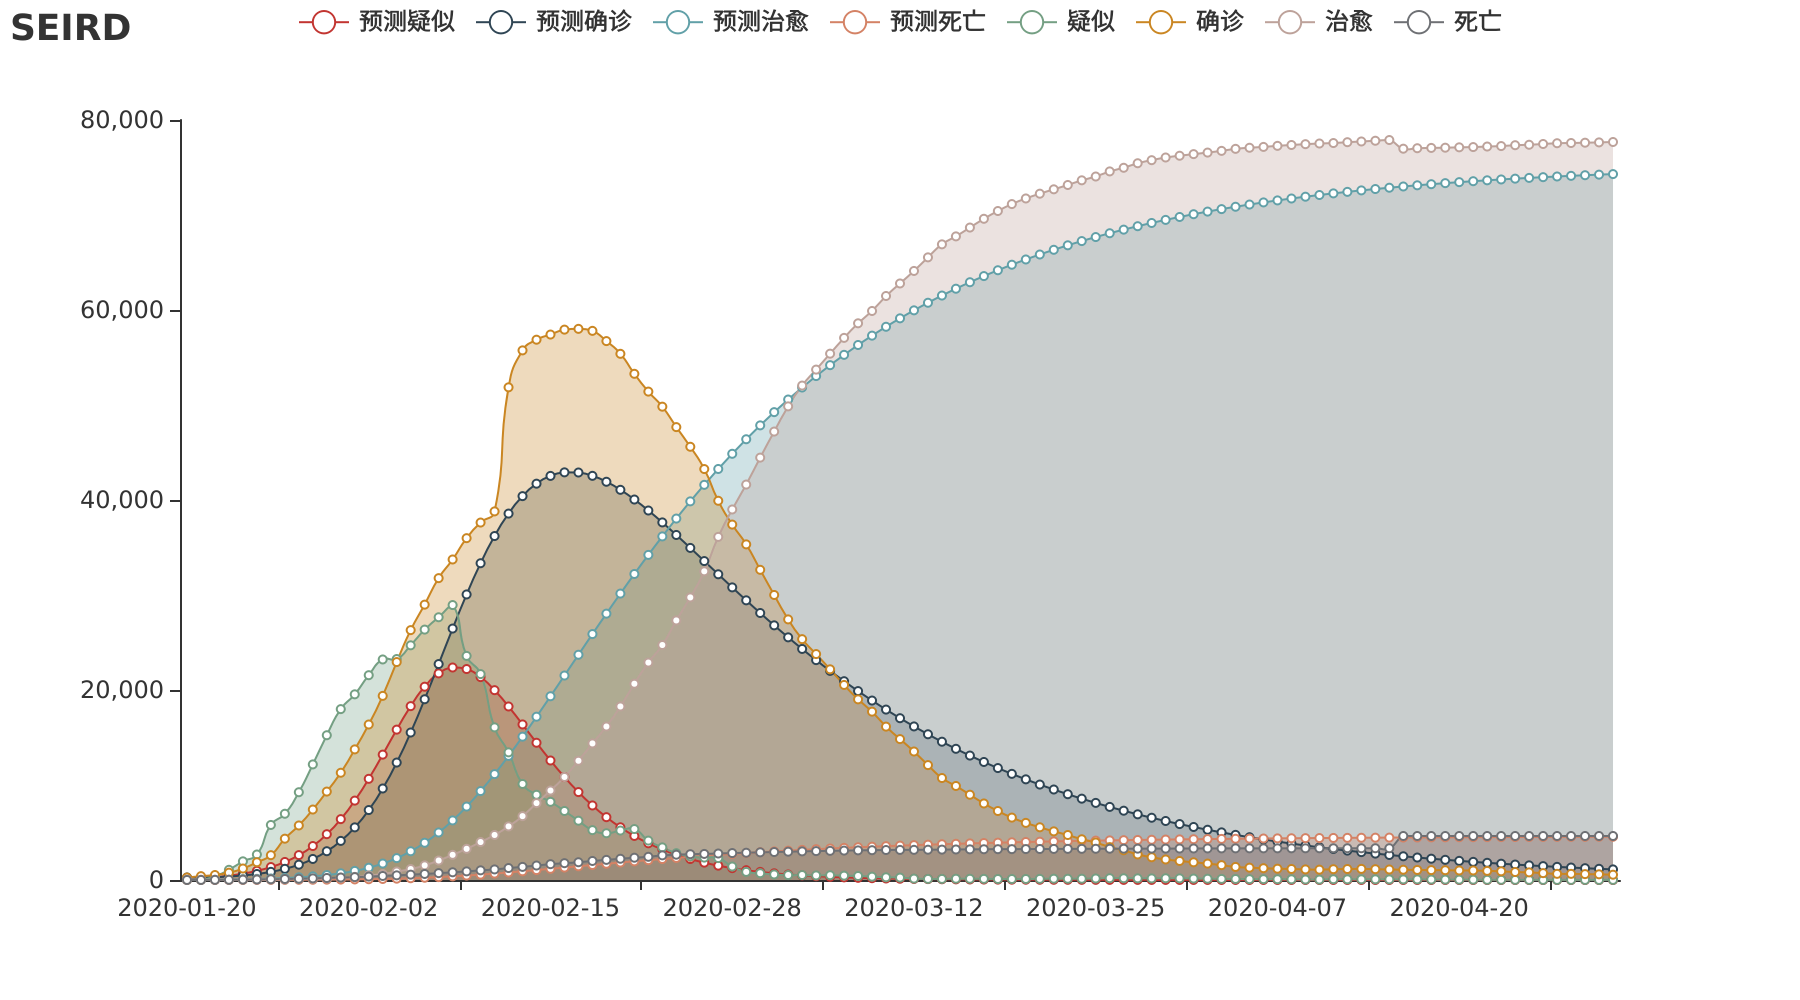
\includegraphics[width=.9\textwidth]{SEIRD.png}
\end{itemize}